\documentclass[12pt,a4paper]{article}
\usepackage[utf8]{inputenc}
\usepackage[T1]{fontenc}
\usepackage{amsmath}
\usepackage{amsfonts}
\usepackage{amssymb}
\usepackage{graphicx}
\usepackage{authblk}

\graphicspath{{./img/}}

\usepackage{times}

\begin{document}

\section*{Mathematical modelling}

Broadly speaking, a mathematical or \textit{in silico} model describes a biological system by a number of independent and dependent variables and a set of equations or rules relating them that govern the state of the system.
When designing an \textit{in silico} model, one has to make choices among the variety of model types available.
This choice is informed by the system to be modelled, the question to be answered and the resources available (e.g., data or computational resources).
Because biological systems are so complex, the mechanisms modelled need to be kept to a minimum in order for the simulations to be tractable and interpretable.
The process of designing and refining an \textit{in silico} model follows a logic similar to experimental sciences and is summarised in Figure~\ref{fig:ModellingCycle}.
In this section, we give a brief overview of different model types that can be used to model the retina and typical challenges emerging when modelling biological systems.
A more comprehensive overview can be found in the work of Roberts et al.\cite{Roberts_2016}

\begin{figure}[ht!]
  \centering
  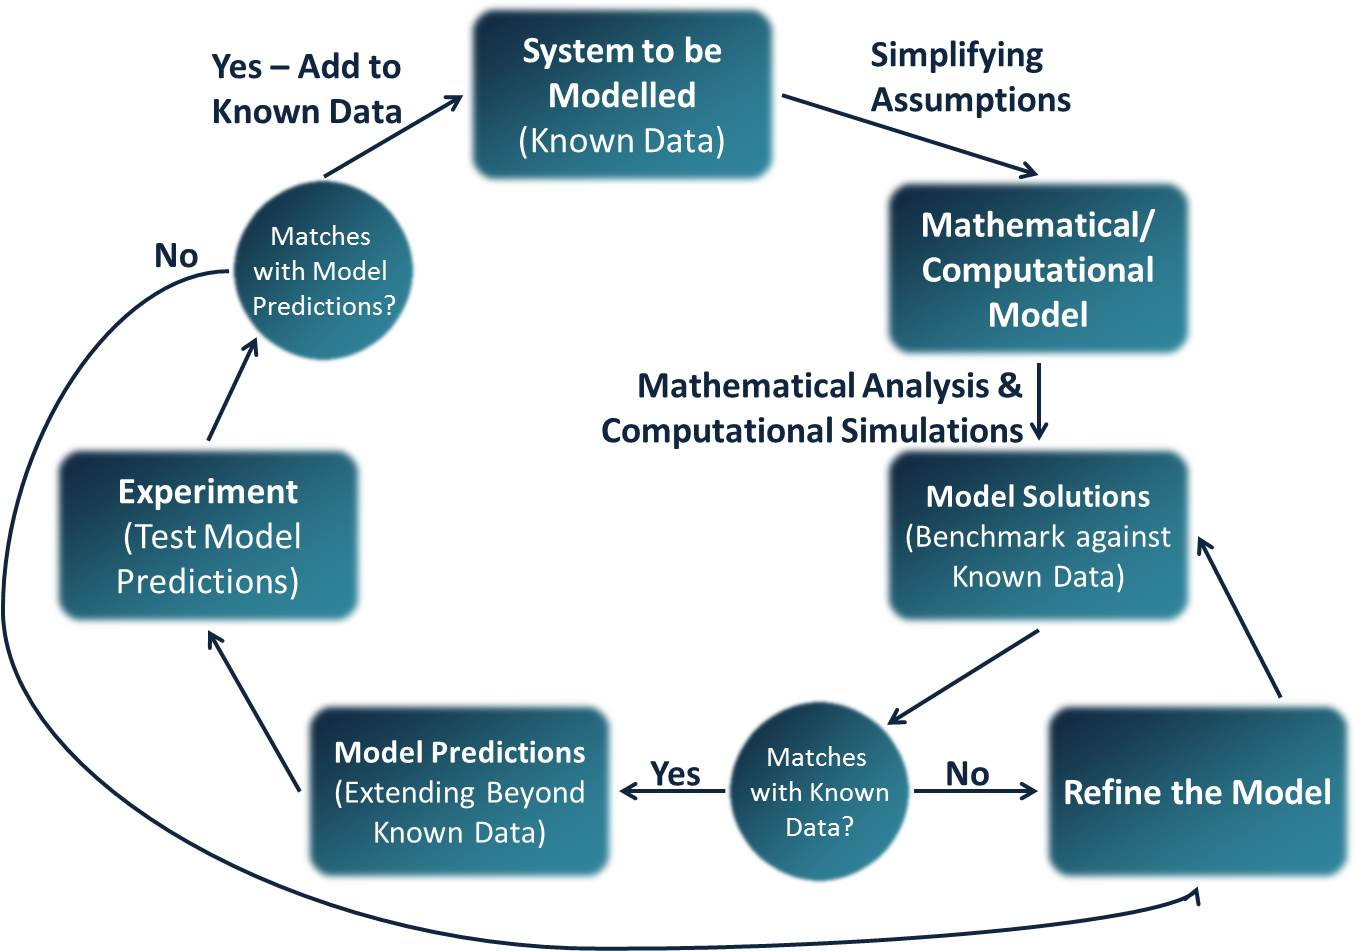
\includegraphics[width=.9\linewidth]{ModellingCycle}
  \caption{Modelling cycle of the design of an \textit{in silico} model. Reused with permission from Roberts et al.\cite{Roberts_2016}}
  \label{fig:ModellingCycle}
\end{figure}

\subsubsection*{Mechanistic vs phenomenological models}
\textit{A priori} understanding of the system can be used to inform model design, in which case the model is qualified as mechanistic.
If appropriate assumption are made, the predictions of a mechanistic model will match observations.
Else, the \textit{a priori} assumptions may need to be reviewed and the model changed accordingly until satisfying agreement is found.
In contrast, phenomenological models simulate parts or the entirety of the system by arbitrary function based on observation of the data.
For instance, an exponential decay is often assumed for time course of drug in the body.
Phenomenological models are often used to simplify an overly complex or unknown mechanism acting on the system to be modelled.
It should be noted that simplifications are inherent to model development and, therefore, no model is fully mechanistic.

All models involve a number of parameters.
Some of those parameters may be known, either from direct measurements or theoretical formulae.
However, other may be unknown because they cannot be measured or are model-specific and may not represent a measurable, physical quantity.
In such cases, \textit{in silico} models can provide estimates of the physical quantity by fitting parameters to data, when available.
Otherwise, analysis of the model predictions may still provide useful insights on the system's behaviour.
Indeed, in either cases, tools such sensitivity analysis and bifurcation analysis can provide insights on the system's behaviour for different parameter regimes.
Known parameters for a simulation may be included as strength of one of the mechanisms, e.g., diffusion speed of a chemical, or incorporated in the model as initial or boundary conditions.

\subsubsection*{Initial and boundary conditions}
While initial boundary conditions are the state of the system at time $t=0$, boundary conditions define the behaviour of the system at the boundaries of a spatial domain.
Classical boundary conditions may set the value of the simulated function itself and is referred to as a Dirichlet boundary condition, of its normal derivative along the boundary, in which case it is called a Neumann boundary condition, or a linear combination of the previous two types, to form a Robin boundary condition.
Up to few exceptions, initial and boundary conditions are necessary for differential equations to be well-posed and solvable.

\subsubsection*{Deterministic and stochastic models}

When random events are left out of a model, two simulations will yield the same results.
This kind of model is referred to as deterministic.
In opposition, stochastic models include a probabilistic component, e.g., the random movement of cells, which yields different solutions for each simulation.
Stochastic models are often used for discrete models.
Discrete models simulate the behaviour of individual entities, such as cells, based on a set of arbitrary rules.
While discrete models can incorporate more details, continuum models allow for rigorous mathematical analysis.
Further limitation of discrete models include the drastic increase in computation times as the number of objects simulated increase.

\subsubsection*{Differential equations}

Many models describe the spatial and temporal behaviour of a quantity within a biological system using differential equations.
Differential equations relate one or more unknown functions with their derivatives.
If the equation involves derivatives with respect to a single independent variable, it is referred to as an ordinary differential equation.
Otherwise, if more than one type of derivative appears in the equation, it is referred to as a partial differential equation.
Differential equations are mathematically tractable and can be solved analytically, when an algebraic expression of the unknown function is found, or numerically.

Partial differential equations often arise when the spatial distribution of the quantity of interest is needed.
However, the spatial aspect is not always relevant to the research question being investigated.
In such cases, an ordinary differential equation relating a function and its time derivative can be used.
Ordinary differential equations can also be used to model a system along of a single spatial dimension at resting, or steady, state.

Assuming a steady state is a common simplifying assumption which can help reduce the complexity and increase the interpretability of the system by ridding the model of the time component.
This reduction follows from assuming that the system, when not perturbed, does not change over time, hence the time derivative of the functions describing it are null.
Similarly, spatial derivatives can be suppressed by assuming that the quantity is homogeneously distributed within the space.
This simplification, referred to in certain context as a well-mixed assumption, is often used to derive compartment models.

Compartmental models describe a system as separated compartments that can interact with each other, e.g., drug concentration in the eye can be described by a vitreal, retinal and choroidal compartment, with mass exchanges between adjacent compartments.
Likewise, lumped parameter models simplify systems with certain spatially distributed objects, such as blood flow within a network of capillaries.
In such models, the spatial aspect is reduced to a smaller number of entities to which the smaller objects are assigned, similarly to how capillaries are grouped into capillary plexi.
To each entity is attached a number of parameters which encompass the various properties of the spatially distributed system.
In the capillary blood flow example, these properties could include vascular resistance, oxygen extraction or storage capacity within each capillary of the network.
Both compartmental models and lumped parameters models describe the system with a set of ordinary differential equations for each of the compartments or entities.

Systems of ordinary differential equations are typically simpler to solve, both analytically and numerically, and to mathematically analyse compared to partial differential equations.
Challenges in the analysis of partial differential equations arise from the possibly complex geometry of biological systems.
Approximating the geometry with simpler shapes such as spheres and rectangles, may allow derivation of analytical solutions or, at least, greatly reduce the time needed to numerically solve the equations.

Numerically, differential equations are solved by discretising (that is, reducing the continuous variable to a finite number of points) the space and time variables into a mesh, at the corner of which the unknown's value is found by solving a matrix equation.
The size of the matrix depends on the refinement of the mesh, with smaller mesh sizes yielding larger matrices.
Therefore, mesh size provides some degree of control over the computational complexity of the model, that is the time and memory needed to run a simulation.

Still, systems with multiple or spatial scales, which often arise in biology, can be challenging to solve within reasonable times.
Indeed, smaller scales enforce smaller mesh sizes in order to account for the refined details of the geometry or of the mechanisms working on different time scales.
This issue appears, for example, when modelling the delivery of oxygen from retinal capillaries to a slab of tissue.
While the size of the tissue may be of the order of millimetres, the numerous blood vessels are, in contrast, of the order of micrometres, hence enforcing a mesh size of the order of micrometres.
In such problems where separate mechanisms interact with each other (e.g., oxygen transport in the capillaries and oxygen diffusion in the tissue), the unknown functions appear in more than one equation.
The model is then said to be coupled.
While coupling adds to the difficulty of solving the equations, clever mathematical techniques may help in reducing the complexity.
However, those tricks are often problem-specific and hard to generalise.

In addition, the often nonlinear behaviour of biological processes can affect the computational cost of running simulations.
Indeed, solving nonlinear equations most often requires to solve a series of subproblems until the difference between successive iterations becomes small enough.

When complex nonlinearities are combined with multiple scales, the time required to solve a set of equations increases dramatically.
For those reasons, computation time remains a barrier to the use of \textit{in silico} models for real-time simulations in the clinic.

\end{document}